\documentclass[hyperref,]{ctexart}
\usepackage{lmodern}
\usepackage{amssymb,amsmath}
\usepackage{ifxetex,ifluatex}
\usepackage{fixltx2e} % provides \textsubscript
\ifnum 0\ifxetex 1\fi\ifluatex 1\fi=0 % if pdftex
  \usepackage[T1]{fontenc}
  \usepackage[utf8]{inputenc}
\else % if luatex or xelatex
  \ifxetex
    \usepackage{xltxtra,xunicode}
  \else
    \usepackage{fontspec}
  \fi
  \defaultfontfeatures{Mapping=tex-text,Scale=MatchLowercase}
  \newcommand{\euro}{€}
\fi
% use upquote if available, for straight quotes in verbatim environments
\IfFileExists{upquote.sty}{\usepackage{upquote}}{}
% use microtype if available
\IfFileExists{microtype.sty}{%
\usepackage{microtype}
\UseMicrotypeSet[protrusion]{basicmath} % disable protrusion for tt fonts
}{}
\ifxetex
  \usepackage[setpagesize=false, % page size defined by xetex
              unicode=false, % unicode breaks when used with xetex
              xetex]{hyperref}
\else
  \usepackage[unicode=true]{hyperref}
\fi
\usepackage[usenames,dvipsnames]{color}
\hypersetup{breaklinks=true,
            bookmarks=true,
            pdfauthor={蓝海; 彭莉},
            pdftitle={分析曹名长-技术报告},
            colorlinks=true,
            citecolor=blue,
            urlcolor=blue,
            linkcolor=magenta,
            pdfborder={0 0 0}}
\urlstyle{same}  % don't use monospace font for urls
\usepackage{longtable,booktabs}
\usepackage{graphicx,grffile}
\makeatletter
\def\maxwidth{\ifdim\Gin@nat@width>\linewidth\linewidth\else\Gin@nat@width\fi}
\def\maxheight{\ifdim\Gin@nat@height>\textheight\textheight\else\Gin@nat@height\fi}
\makeatother
% Scale images if necessary, so that they will not overflow the page
% margins by default, and it is still possible to overwrite the defaults
% using explicit options in \includegraphics[width, height, ...]{}
\setkeys{Gin}{width=\maxwidth,height=\maxheight,keepaspectratio}
\setlength{\emergencystretch}{3em}  % prevent overfull lines
\providecommand{\tightlist}{%
  \setlength{\itemsep}{0pt}\setlength{\parskip}{0pt}}
\setcounter{secnumdepth}{5}

\title{分析曹名长-技术报告}
\author{蓝海 \and 彭莉}
\date{}

% Redefines (sub)paragraphs to behave more like sections
\ifx\paragraph\undefined\else
\let\oldparagraph\paragraph
\renewcommand{\paragraph}[1]{\oldparagraph{#1}\mbox{}}
\fi
\ifx\subparagraph\undefined\else
\let\oldsubparagraph\subparagraph
\renewcommand{\subparagraph}[1]{\oldsubparagraph{#1}\mbox{}}
\fi

\begin{document}
\maketitle

{
\setcounter{tocdepth}{2}
\tableofcontents
}
\section{业绩表现}

\subsection{曹名长}

历任君安证券公司研究所研究员,闽发证券上海研发中心研究员,红塔证券资产管理总部投资经理,百瑞信托有限责任公司信托经理,新华基金管理公司总经理助理、基金经理。2015年6月加入中欧基金管理有限公司,现任事业部负责人、基金经理。

曹名长前后共管理过8个不同的基金产品,有些基金创设时间太短,不具备分析价值,所以我们重点的挑选了4只基金为代表进行分析。两支正在中欧基金管理的基金:中欧价值发现混合A和中欧潜力价值灵活配置混合;两支之前在新华基金管理的基金:新华钻石品质企业混合和新华优选分红混合。

\subsection{当前表现}

\begin{figure}[htbp]
\centering
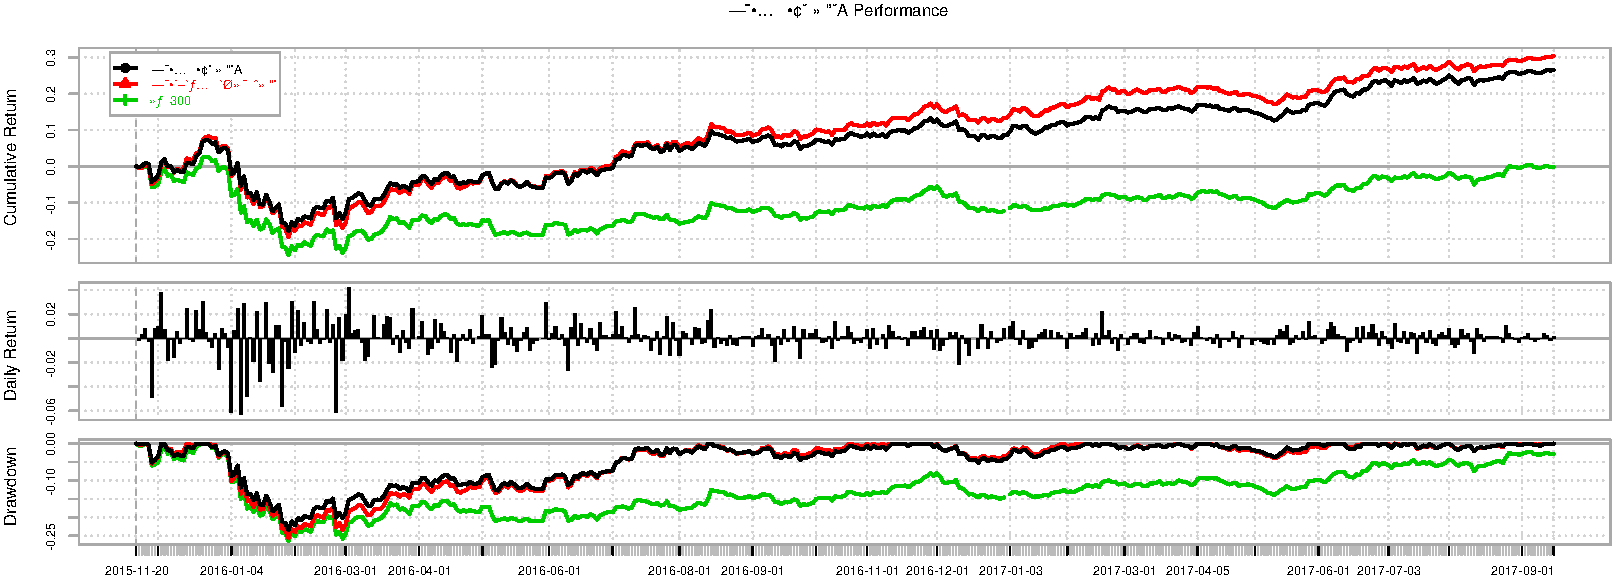
\includegraphics{caominchang-details_files/figure-latex/unnamed-chunk-1-1.pdf}
\caption{基金累计回报率与回撤}
\end{figure}

\begin{longtable}[]{@{}llclclc@{}}
\toprule
名称 & 近半年 & 夏普率 & 近一年 & 夏普率 & 近两年 &
夏普率\tabularnewline
\midrule
\endhead
中欧价值发现混合A & 9.3\% & 1.9 & 18\% & 0.61 & 26.6\% &
0.53\tabularnewline
中欧潜力价值灵活配置混合 & 7.8\% & 1.6 & 20\% & 0.69 & 30.4\% &
0.61\tabularnewline
沪深300 & 8.9\% & 1.5 & 14\% & -0.14 & -0.2\% & -0.21\tabularnewline
\bottomrule
\end{longtable}

\begin{figure}[htbp]
\centering
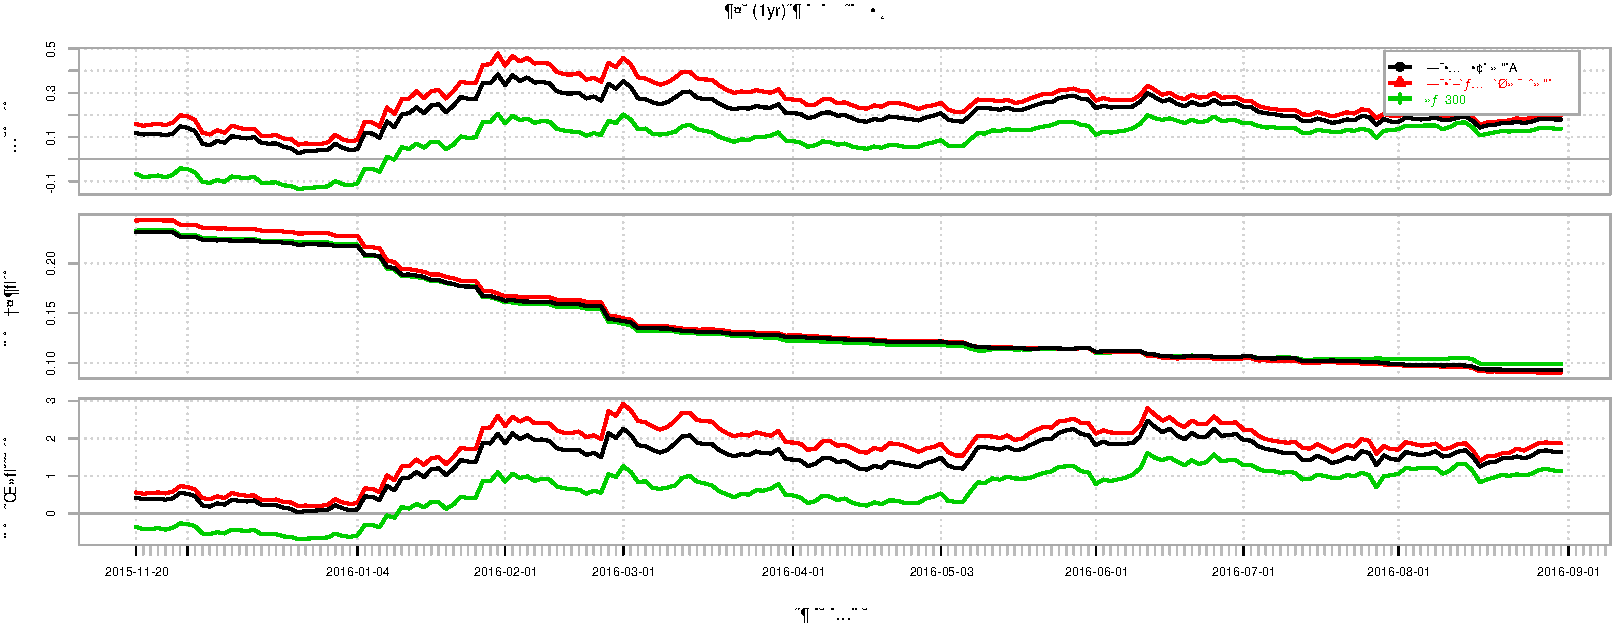
\includegraphics{caominchang-details_files/figure-latex/unnamed-chunk-2-1.pdf}
\caption{投资者收益风险比较}
\end{figure}

图1清楚的表明自曹名长在管理该两支基金以来相对于沪深300其累计收益率的不俗表现。同时在风险控制方面,除了2016年初的股灾2.0期间回撤相当之外,其他时候该两支基金的回撤都显著小于对应时期的沪深300的回撤,显示了良好的风险控制能力。图2明确的表明,固定一年期的投资者,无论何时买入这两只基金,他都可以获得相比沪深300更高的累计收益,并且日收益序列的风险收益比------夏普率------都是显著高于沪深300的。通俗的说,就是不但能够赚更多的钱,而且作为投资者,你还更有可能``拿得住''这样的投资对象,因为波动更小。表1以回溯的方式明确的显示了两支基金的相对优势。
以上可见加入中欧基金以来,曹名长在管理的两支基金上都取得了不俗的业绩。

\subsection{历史表现}

曾经在新华基金管理过的基金产品在其管理期间的表现为:
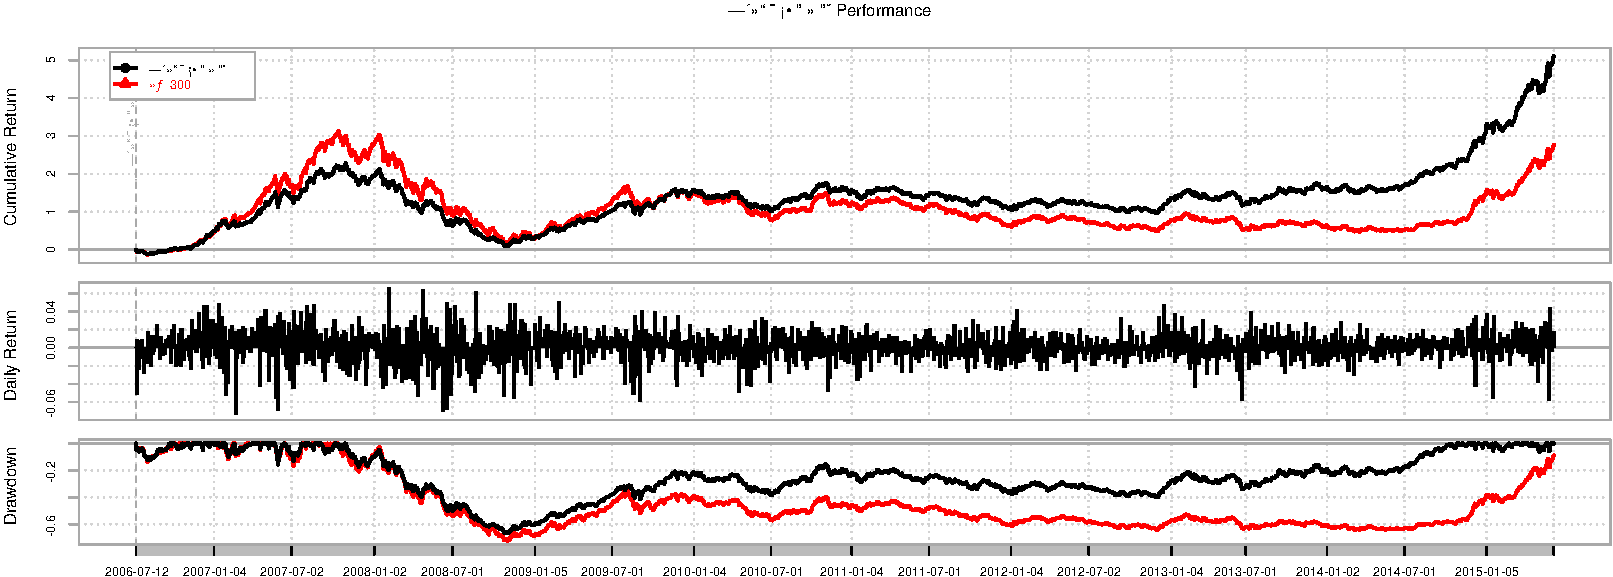
\includegraphics{caominchang-details_files/figure-latex/unnamed-chunk-3-1.pdf}
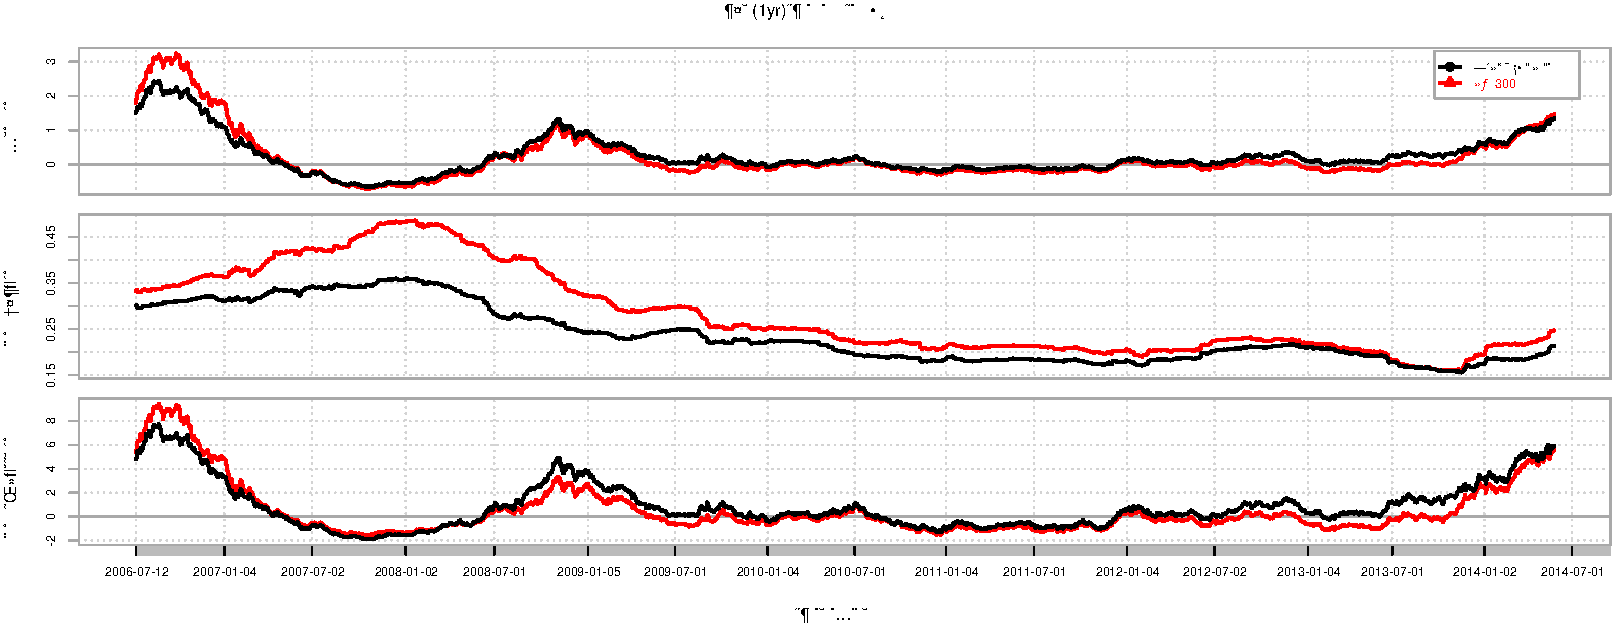
\includegraphics{caominchang-details_files/figure-latex/unnamed-chunk-3-2.pdf}
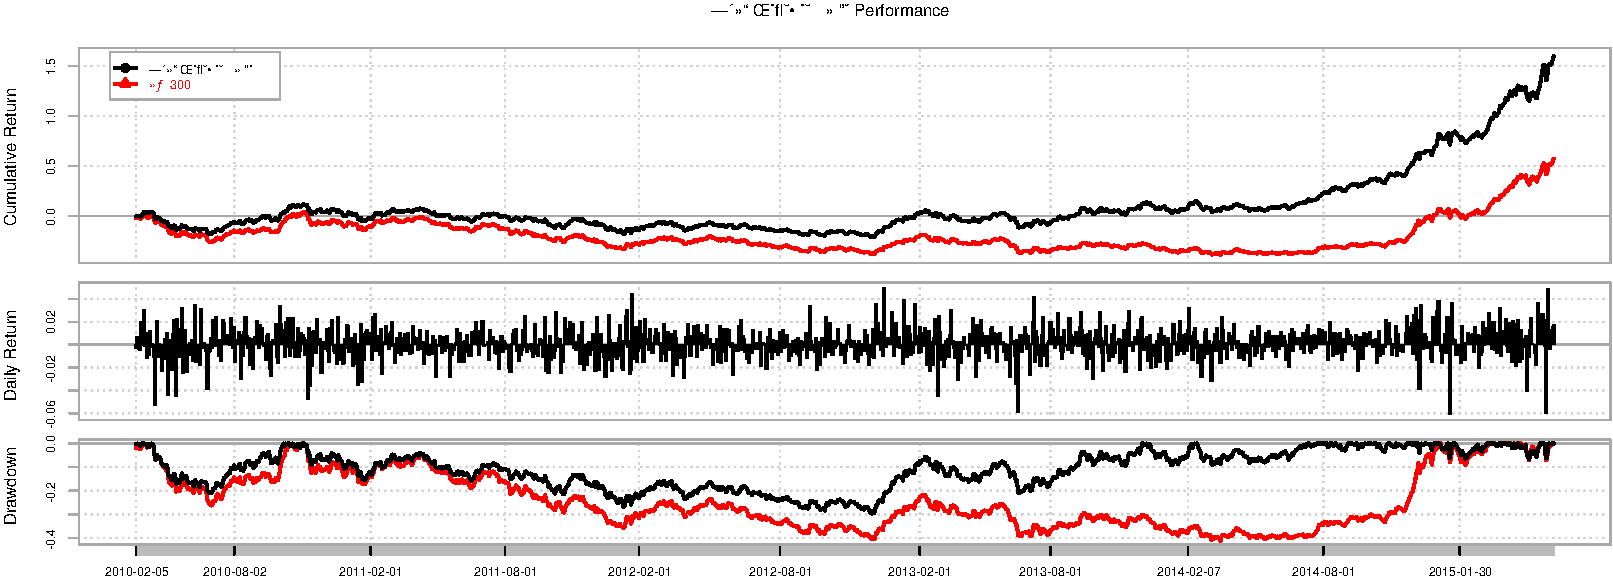
\includegraphics{caominchang-details_files/figure-latex/unnamed-chunk-3-3.pdf}
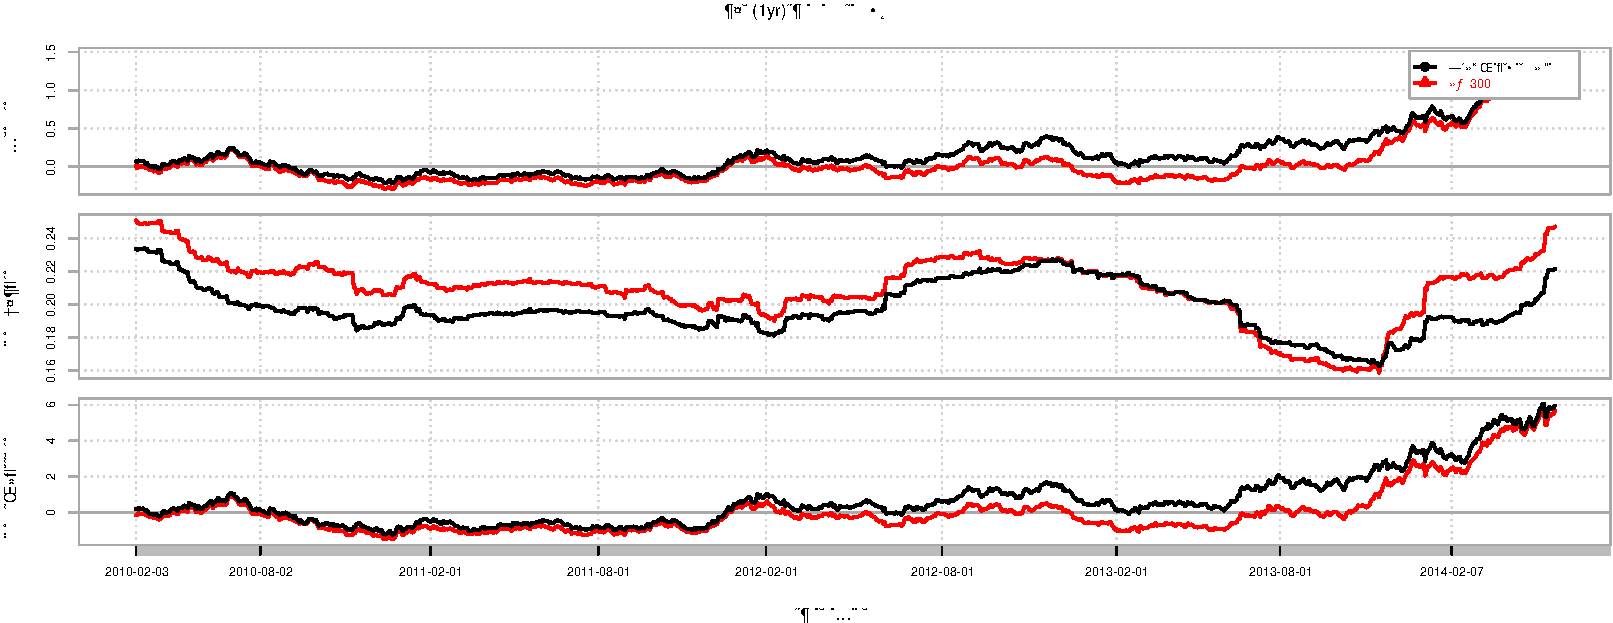
\includegraphics{caominchang-details_files/figure-latex/unnamed-chunk-3-4.pdf}

\begin{longtable}[]{@{}llclclclc@{}}
\toprule
名称 & 最后半年 & 夏普率 & 一年 & 夏普率 & 两年 & 夏普率 & 三年 &
夏普率\tabularnewline
\midrule
\endhead
新华优选分红混合 & 68\% & 6.5 & 135\% & 5.9 & 156\% & 2.7 & 171\% &
1.7\tabularnewline
新华钻石品质企业混合 & 70\% & 6.4 & 140\% & 5.9 & 166\% & 2.7 & 186\% &
1.7\tabularnewline
沪深300 & 91\% & 7.8 & 148\% & 5.6 & 112\% & 1.8 & 105\% &
1.0\tabularnewline
\bottomrule
\end{longtable}

依旧可以看到,曹名长在长达9年的新华基金工作期间,其管理的基金在多数时候绝对收益超过沪深300,并且波动率小于参照。如投资者固定投资其管理的基金一年,大多数时候投资都会有正的收益(但是,绝对收益有负的情况。就是虽然跑过了市场,但是市场实在太糟!),并且持有期间的收益风险比好于沪深300。表2显示的其离开新华前3年的超乎常理的亮眼表现,更多的是来自2014-2015年中国市场的一波``疯牛''市,不可简单推论。

\section{风格分析}

\subsection{交易风格}

基于公开信息,我们对曹名长的正在管理的中欧潜力价值灵活配置混合的交易风格分析如下:

\begin{longtable}[]{@{}lcccccc@{}}
\toprule
日期 & 换手率 & 排名\% & 持有期 & 排名\% & 前十占比\% &
排名\%\tabularnewline
\midrule
\endhead
2015 Q4 & 336 & 85 & NA & 0 & 34 & 90\tabularnewline
2016 Q2 & 67 & 90 & 0.76 & 31 & 28 & 94\tabularnewline
2016 Q4 & 130 & 94 & NA & 0 & 28 & 92\tabularnewline
\bottomrule
\end{longtable}

\begin{longtable}[]{@{}lccccrcrc@{}}
\toprule
日期 & 行业前5占比\% & 排名\% & 平均集中度 & 排名\% & PE & 排名\% & PB &
排名\%\tabularnewline
\midrule
\endhead
2015 Q4 & 96 & 47 & 0.05 & 70 & 15 & 89 & 2.1 & 90\tabularnewline
2016 Q2 & 95 & 60 & 0.03 & 74 & 11 & 93 & 1.7 & 90\tabularnewline
2016 Q4 & 93 & 65 & 0.05 & 53 & 14 & 78 & 1.9 & 74\tabularnewline
\bottomrule
\end{longtable}

其中排名,从0到100\%,是按照对应数值从高到低的顺序,在同期同类基金中做出的。比如前10占比排名在20\%左右,意味着其相对与一般混合式基金持有股票的前10占比比较小于约80\%的基金。但是,该基金的行业集中度处于同类型基金的中间水平,换手率低于同类基金\footnote{因为基金经营时间不长,没有足够的报告数据,因此持有期数据仅有一次有价值的数据,读者对于这样的数据当谨慎怀疑。不过配合总换手率的数据,我们推论其持有期较长,是合理的。}。从以上表格中可以看出
\emph{中欧潜力价值灵活配置混合基金,是以非常低的换手率,长期地投资于低PB和低PE的股票来获取收益的}。

同样的对于早期在新华基金管理了接近9年的新华优选分红混合基金进行交易风格分析,我们也发现了相似的情况。数据如下:

\begin{longtable}[]{@{}lcccccc@{}}
\toprule
日期 & 换手率 & 排名\% & 持有期 & 排名\% & 前十占比\% &
排名\%\tabularnewline
\midrule
\endhead
2010 Q2 & 113 & 68 & 0.42 & 43 & 56 & 23\tabularnewline
2010 Q4 & 245 & 69 & 0.20 & 52 & 55 & 17\tabularnewline
2011 Q2 & 75 & 78 & 0.69 & 28 & 61 & 11\tabularnewline
2011 Q4 & 129 & 84 & 0.41 & 30 & 57 & 25\tabularnewline
2012 Q2 & 48 & 90 & 1.05 & 15 & 57 & 21\tabularnewline
2012 Q4 & 94 & 92 & 0.55 & 20 & 57 & 23\tabularnewline
2013 Q2 & 78 & 87 & 0.61 & 21 & 61 & 24\tabularnewline
2013 Q4 & 157 & 87 & 0.33 & 23 & 59 & 31\tabularnewline
2014 Q2 & 59 & 89 & 0.88 & 21 & 60 & 32\tabularnewline
2014 Q4 & 128 & 92 & 0.51 & 23 & 42 & 78\tabularnewline
2015 Q2 & 141 & 85 & 0.31 & 36 & 52 & 66\tabularnewline
\bottomrule
\end{longtable}

\begin{longtable}[]{@{}lccccrcrc@{}}
\toprule
日期 & 行业前5占比\% & 排名\% & 平均集中度 & 排名\% & PE & 排名\% & PB &
排名\%\tabularnewline
\midrule
\endhead
2010 Q2 & 86 & 7 & 0.56 & 58 & 16.4 & 68 & 3.5 & 54\tabularnewline
2010 Q4 & 81 & 9 & 0.25 & 75 & 21.6 & 82 & 3.2 & 89\tabularnewline
2011 Q2 & 76 & 26 & 0.71 & 42 & 17.5 & 59 & 2.8 & 82\tabularnewline
2011 Q4 & 76 & 28 & 0.81 & 41 & 16.1 & 52 & 2.1 & 83\tabularnewline
2012 Q2 & 87 & 7 & 0.22 & 63 & 12.3 & 84 & 2.0 & 89\tabularnewline
2012 Q4 & 79 & 22 & 0.84 & 29 & 13.8 & 66 & 2.0 & 75\tabularnewline
2013 Q2 & 87 & 87 & 0.81 & 29 & 8.2 & 96 & 1.4 & 97\tabularnewline
2013 Q4 & 91 & 76 & 1.04 & 24 & 11.2 & 91 & 1.6 & 94\tabularnewline
2014 Q2 & 93 & 76 & 0.85 & 29 & 10.6 & 90 & 1.7 & 92\tabularnewline
2014 Q4 & 95 & 44 & 0.52 & 33 & 14.9 & 82 & 2.0 & 89\tabularnewline
2015 Q2 & 96 & 46 & 0.19 & 58 & 14.3 & 93 & 2.3 & 95\tabularnewline
\bottomrule
\end{longtable}

在新华基金期间,其交易风格整体是低换手率,长持有期。尤其是在市场环境不好的2011-2012年间,换手率极低,显示出其超强的抗压能力。

\begin{longtable}[]{@{}lcccccc@{}}
\toprule
日期 & 换手率 & 排名\% & 持有期 & 排名\% & 前十占比\% &
排名\%\tabularnewline
\midrule
\endhead
2010 Q2 & 367 & 9 & NA & 0 & 59 & 16\tabularnewline
2010 Q4 & 374 & 44 & NA & 0 & 56 & 13\tabularnewline
2011 Q2 & 77 & 76 & 0.69 & 29 & 63 & 8\tabularnewline
2011 Q4 & 132 & 83 & 0.41 & 30 & 61 & 16\tabularnewline
2012 Q2 & 57 & 86 & 0.88 & 20 & 57 & 21\tabularnewline
2012 Q4 & 135 & 82 & 0.38 & 29 & 56 & 27\tabularnewline
2013 Q2 & 106 & 76 & 0.46 & 30 & 59 & 29\tabularnewline
2013 Q4 & 196 & 80 & 0.26 & 31 & 59 & 31\tabularnewline
2014 Q2 & 75 & 85 & 0.70 & 26 & 59 & 33\tabularnewline
2014 Q4 & 134 & 92 & 0.50 & 23 & 40 & 83\tabularnewline
2015 Q2 & 116 & 91 & 0.37 & 31 & 54 & 58\tabularnewline
\bottomrule
\end{longtable}

\begin{longtable}[]{@{}lccccrcrc@{}}
\toprule
日期 & 行业前5占比\% & 排名\% & 平均集中度 & 排名\% & PE & 排名\% & PB &
排名\%\tabularnewline
\midrule
\endhead
2010 Q2 & 89 & 4 & 0.49 & 60 & 15.1 & 74 & 3.3 & 59\tabularnewline
2010 Q4 & 83 & 7 & 0.20 & 80 & 22.4 & 79 & 3.2 & 89\tabularnewline
2011 Q2 & 79 & 19 & 0.89 & 32 & 18.3 & 54 & 2.9 & 80\tabularnewline
2011 Q4 & 80 & 20 & 1.26 & 25 & 17.4 & 46 & 2.2 & 81\tabularnewline
2012 Q2 & 85 & 11 & 0.12 & 76 & 11.4 & 88 & 1.9 & 91\tabularnewline
2012 Q4 & 76 & 32 & 0.49 & 42 & 14.0 & 64 & 2.0 & 74\tabularnewline
2013 Q2 & 92 & 61 & 0.37 & 49 & 8.7 & 95 & 1.5 & 95\tabularnewline
2013 Q4 & 91 & 77 & 0.48 & 43 & 12.9 & 87 & 1.7 & 93\tabularnewline
2014 Q2 & 93 & 74 & 0.45 & 44 & 11.2 & 89 & 1.7 & 92\tabularnewline
2014 Q4 & 95 & 46 & 0.32 & 42 & 15.2 & 81 & 2.0 & 89\tabularnewline
2015 Q2 & 96 & 49 & 0.08 & 75 & 13.7 & 94 & 2.2 & 96\tabularnewline
\bottomrule
\end{longtable}

当然,曹名长的交易风格也并非一成不变的,如上表所示,在基金产品创建初期,又适逢市场环境不好,他也进行过频繁的操作,虽然没有积累较多的正收益,但是跑赢了当期沪深300指数。同时也看到,在新华时期,曹名长投资的股票的PB和PE都高于他最近在中欧管理股票的PB和PE。绝对值的降低,可以由市场估值回归来解释,但是在同类基金中投资股票的平均PB和PE的排名降低,就不得不说这是管理者主动适应市场风格变化的举动了。

\subsection{持仓风格}

基于净值数据,我们对曹名长在中欧基金以及新华基金中的四支基金的持仓风格分析如下。

\subsubsection{中欧价值发现混合A}\label{a}

\begin{longtable}[]{@{}cccc@{}}
\caption{持仓风格权重分析(\%)}\tabularnewline
\toprule
大盘价值 & 小盘价值 & 债券财富指数 & 货币\tabularnewline
\midrule
\endfirsthead
\toprule
大盘价值 & 小盘价值 & 债券财富指数 & 货币\tabularnewline
\midrule
\endhead
51 & 42 & 2.1 & 5\tabularnewline
\bottomrule
\end{longtable}

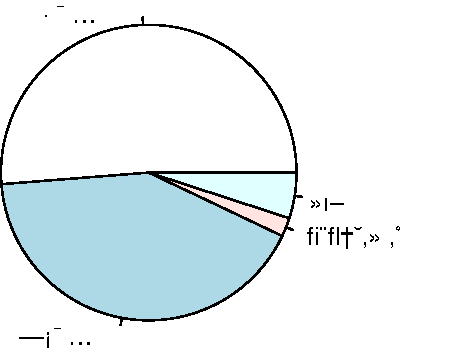
\includegraphics{caominchang-details_files/figure-latex/unnamed-chunk-7-1.pdf}

\subsubsection{中欧潜力价值灵活配置混合}

\begin{longtable}[]{@{}ccc@{}}
\caption{持仓风格权重分析(\%)}\tabularnewline
\toprule
大盘价值 & 小盘价值 & 货币\tabularnewline
\midrule
\endfirsthead
\toprule
大盘价值 & 小盘价值 & 货币\tabularnewline
\midrule
\endhead
44 & 51 & 5\tabularnewline
\bottomrule
\end{longtable}

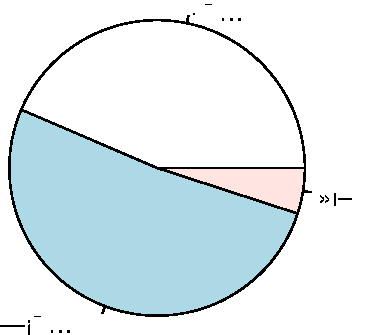
\includegraphics{caominchang-details_files/figure-latex/unnamed-chunk-8-1.pdf}

可见,其重点投资的股票往往都是价值类型的股票,这与当前的市场风格是吻合的。

\subsubsection{新华钻石品质企业混合}

\begin{longtable}[]{@{}cccc@{}}
\caption{持仓风格权重分析(\%)}\tabularnewline
\toprule
大盘价值 & 中盘成长 & 中盘价值 & 货币\tabularnewline
\midrule
\endfirsthead
\toprule
大盘价值 & 中盘成长 & 中盘价值 & 货币\tabularnewline
\midrule
\endhead
31 & 29 & 24 & 16\tabularnewline
\bottomrule
\end{longtable}

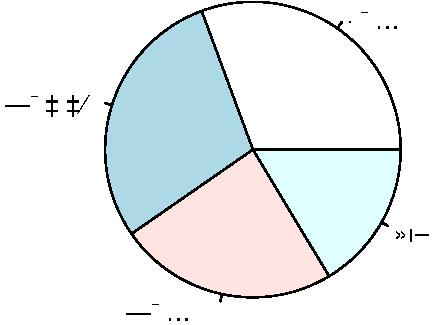
\includegraphics{caominchang-details_files/figure-latex/unnamed-chunk-9-1.pdf}

\subsubsection{新华钻石品质企业混合持仓风格}

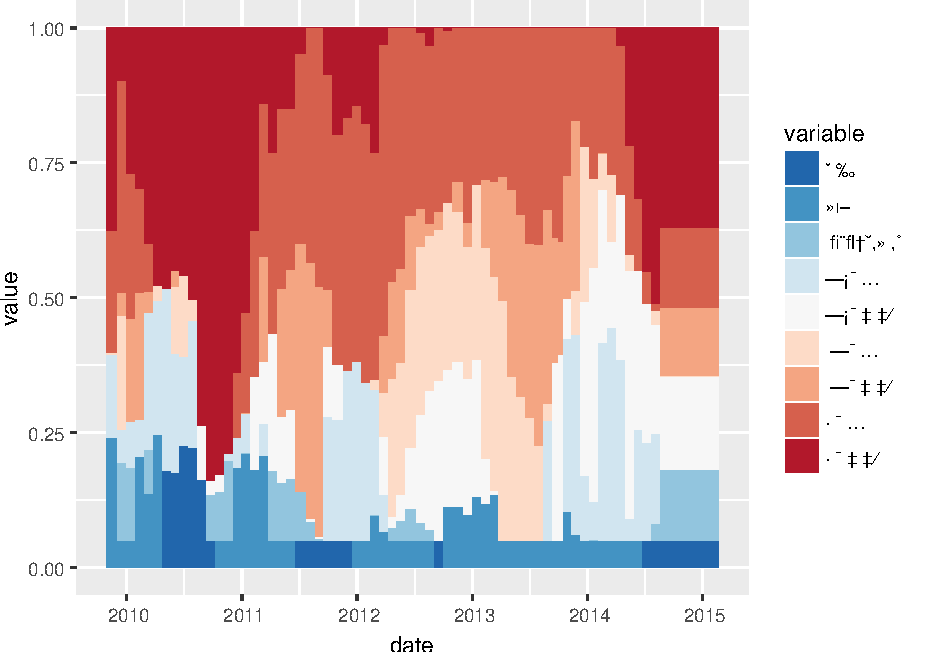
\includegraphics{caominchang-details_files/figure-latex/unnamed-chunk-32-1.pdf}

风格变化较大,如平均占比最高的大盘价值其占比最高53.95\%最低0.00\%

\subsubsection{新华优选分红混合}

\begin{longtable}[]{@{}cccccc@{}}
\caption{持仓风格权重分析(\%)}\tabularnewline
\toprule
大盘成长 & 大盘价值 & 中盘成长 & 小盘价值 & 债券财富指数 &
货币\tabularnewline
\midrule
\endfirsthead
\toprule
大盘成长 & 大盘价值 & 中盘成长 & 小盘价值 & 债券财富指数 &
货币\tabularnewline
\midrule
\endhead
57 & 2.9 & 16 & 3 & 16 & 5\tabularnewline
\bottomrule
\end{longtable}

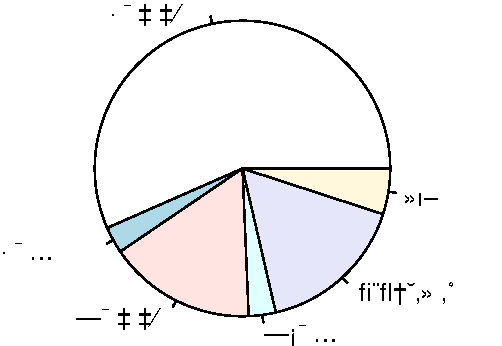
\includegraphics{caominchang-details_files/figure-latex/unnamed-chunk-11-1.pdf}

这两只基金因为存续于不同的时期,所以其风格并不十分类似。但是总体上,相对于他现在正在管理的基金,更多的投资权重放到了成长类型的股票当中。同时这也反映在持有股票的平均PE较大。这种偏重成长类型的风格实际上也贴合了那一段时期,中国市场偏爱创业板、偏爱成长型题材的市场风格。另外曹名长在中欧基金比较其在新华基金期间,持股的行业集中度和前10大股票集中度都有所降低。

从中可见,\emph{曹名长是一个能够跟随市场风格变化而主动变化的,有学习能力的主动投资者}。

\subsection{主动风格:稳健}

我们用行业累计偏离指数代表该基金主动管理的活跃度(在Kacperczyk等的研究中,这个指标又被成为行业集中度)。我们的逻辑根据建立在弱有效市场指数代表了整个市场的``简单''共识,大量的``smart
beta''的机会留给了基金管理人,在追寻``smart
beta''的过程中,突破原有的行业布局不可避免。而这种突破正可以被行业累计偏离指数来捕捉。但是,主动指数并非越大越好,毕竟市场是弱有效的,完全忽略市场的共识------哪怕是``简单''共识------也是唐吉坷德式的挑战风车。实际上有研究表明,基金业绩表现与Kacperczyk的行业集中度呈现负相关,即行业集中度越大,基金表现越差。我们的分析表明,这种联系在中国市场不是简单照搬的,对于极端的行业集中的情形,确实行业集中度越高,基金平均表现越差,但是在一个温和的区间中,这样的联系是不存在的。当然这个主动指数可以进一步的拓展到对包含基金经理追求alpha
的描述,这是我们下一步的工作方向之一。

以其管理的中欧价值发现混合A基金为说明,从创建到其接收管理之前,该基金的平均主动管理活跃度为40.25\%,呈现非常激进的主动管理态势;其接管基金后平均主动管理活跃度为17.62\%,表现为积极但是有限度的主动管理。在其管理的同期,整个基金行业的同类型基金的主动管理活跃指数为27.35\%。因此,\emph{对于曹名长的管理风格可以定义为稳健的主动管理型}。所谓``稳健''是指投资者在跟随市场指数配置的基础上,有限度的依据主观判断,适当的超配或者低配某些行业,获取smart
beta的管理形态。主动指标\(\leq 20\%\),为稳健型。

\section{能力评价}

\subsection{大类资产配置:几乎为零}

从下图可以看出,自从2015年11月接手以来,曹名长在产品中欧价值发现混合A中将股票仓位控制在80-95\%之间,而另外一个产品中欧潜力价值灵活配置混合股票仓位则也类似的在70\%-95\%之间变换。

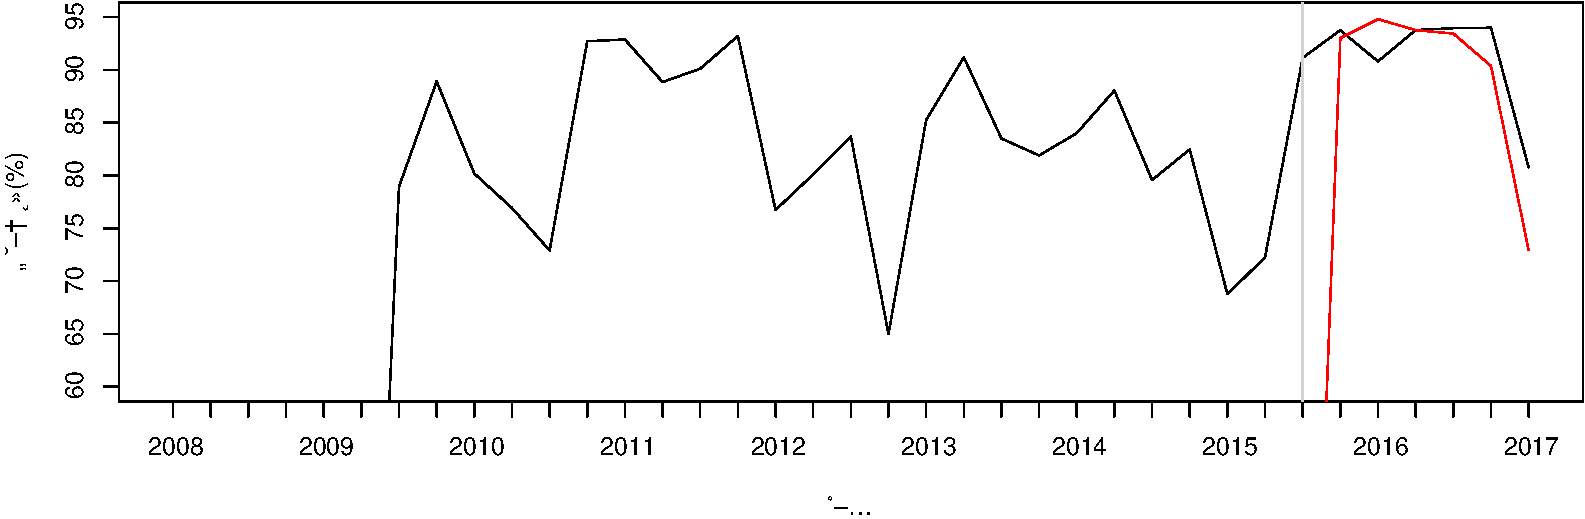
\includegraphics{caominchang-details_files/figure-latex/unnamed-chunk-13-1.pdf}

由于该两个产品管理时间尚且嫌短,我们继续调查他在新华基金时重点管理的另外两支产品新华钻石品质企业混合和新华优选分红混合。

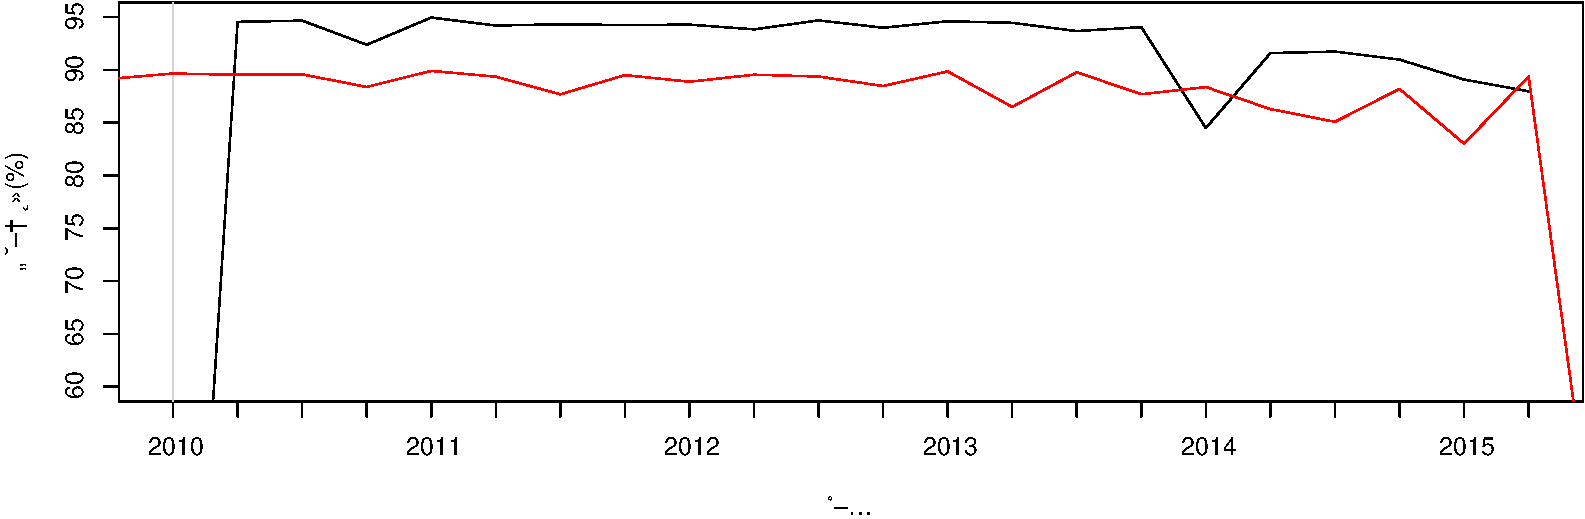
\includegraphics{caominchang-details_files/figure-latex/unnamed-chunk-14-1.pdf}

但是在这两个基金中,他的股票仓位基本都控制在90\%左右,并没有显示主动的仓位调节。

进一步的计算大类资产配置带来的超额收益。

\subsubsection{中欧价值发现混合A}\label{a-1}

\begin{longtable}[]{@{}lc@{}}
\caption{中欧价值发现混合A大类资产配置能力统计}\tabularnewline
\toprule
日期 & 大类资产配置超额贡献(\%)\tabularnewline
\midrule
\endfirsthead
\toprule
日期 & 大类资产配置超额贡献(\%)\tabularnewline
\midrule
\endhead
2015 Q4 & 1.57\tabularnewline
2016 Q1 & -1.86\tabularnewline
2016 Q2 & -0.27\tabularnewline
2016 Q3 & 0.13\tabularnewline
2016 Q4 & 0.59\tabularnewline
2017 Q1 & 0.48\tabularnewline
\bottomrule
\end{longtable}

\begin{longtable}[]{@{}cl@{}}
\toprule
平均超额贡献(\%) & 90\%置信区间\tabularnewline
\midrule
\endhead
0.11 & \([-0.58,\infty)\)\tabularnewline
\bottomrule
\end{longtable}

统计显示,在中欧价值发现混合A这支基金的管理上,虽然每季度平均取得 0.1\%
的配置收益,但是统计意义上并不显著。因此曹名长并没有显示出大类资产配置的能力。

\subsubsection{中欧潜力价值灵活配置混合}\label{-1}

\begin{longtable}[]{@{}lc@{}}
\caption{中欧价值发现混合A大类资产配置能力统计}\tabularnewline
\toprule
日期 & 大类资产配置超额贡献(\%)\tabularnewline
\midrule
\endfirsthead
\toprule
日期 & 大类资产配置超额贡献(\%)\tabularnewline
\midrule
\endhead
2015 Q4 & -2.89\tabularnewline
2016 Q1 & -5.07\tabularnewline
2016 Q2 & -0.82\tabularnewline
2016 Q3 & 0.39\tabularnewline
2016 Q4 & 1.23\tabularnewline
2017 Q1 & 1.21\tabularnewline
\bottomrule
\end{longtable}

\begin{longtable}[]{@{}cl@{}}
\toprule
平均超额贡献\% & 90\%置信区间\tabularnewline
\midrule
\endhead
-0.99 & \([-2.51,\infty)\)\tabularnewline
\bottomrule
\end{longtable}

统计显示,在中欧潜力价值灵活配置混合这支基金的管理上,每季度平均取得
-0.99\% 的配置收益。因此曹名长并没有显示出大类资产配置的能力。

\subsubsection{新华钻石品质企业混合}\label{-1}

\begin{longtable}[]{@{}lc@{}}
\caption{中欧价值发现混合A大类资产配置能力统计}\tabularnewline
\toprule
日期 & 大类资产配置超额贡献(\%)\tabularnewline
\midrule
\endfirsthead
\toprule
日期 & 大类资产配置超额贡献(\%)\tabularnewline
\midrule
\endhead
2010 Q1 & NA\tabularnewline
2010 Q2 & 7.697\tabularnewline
2010 Q3 & 1.973\tabularnewline
2010 Q4 & 1.225\tabularnewline
2011 Q1 & 0.332\tabularnewline
2011 Q2 & -0.842\tabularnewline
2011 Q3 & -2.162\tabularnewline
2011 Q4 & -1.952\tabularnewline
2012 Q1 & 0.566\tabularnewline
2012 Q2 & -0.309\tabularnewline
2012 Q3 & -0.876\tabularnewline
2012 Q4 & 1.339\tabularnewline
2013 Q1 & -0.394\tabularnewline
2013 Q2 & -1.847\tabularnewline
2013 Q3 & 1.578\tabularnewline
2013 Q4 & -0.043\tabularnewline
2014 Q1 & -1.100\tabularnewline
2014 Q2 & -0.417\tabularnewline
2014 Q3 & 1.325\tabularnewline
2014 Q4 & 4.655\tabularnewline
2015 Q1 & 1.427\tabularnewline
2015 Q2 & 0.560\tabularnewline
\bottomrule
\end{longtable}

\begin{longtable}[]{@{}cl@{}}
\toprule
平均超额贡献\% & 90\%置信区间\tabularnewline
\midrule
\endhead
0.61 & \([-0.05,\infty)\)\tabularnewline
\bottomrule
\end{longtable}

统计显示,在新华钻石品质企业混合这支基金的管理上,虽然每季度平均取得
0.61\%
的配置收益,但是统计意义上并不显著。因此无法肯定曹名长大类资产配置的能力。

\subsubsection{新华优选分红混合}\label{-1}

\begin{longtable}[]{@{}lc@{}}
\caption{中欧价值发现混合A大类资产配置能力统计}\tabularnewline
\toprule
日期 & 大类资产配置超额贡献(\%)\tabularnewline
\midrule
\endfirsthead
\toprule
日期 & 大类资产配置超额贡献(\%)\tabularnewline
\midrule
\endhead
2008 Q1 & NA\tabularnewline
2008 Q2 & -4.66\tabularnewline
2008 Q3 & -1.91\tabularnewline
2008 Q4 & -1.23\tabularnewline
2009 Q1 & 9.58\tabularnewline
2009 Q2 & 7.68\tabularnewline
2009 Q3 & -1.35\tabularnewline
2009 Q4 & 5.42\tabularnewline
2010 Q1 & -2.46\tabularnewline
2010 Q2 & -7.26\tabularnewline
2010 Q3 & 4.01\tabularnewline
2010 Q4 & 2.46\tabularnewline
2011 Q1 & 0.71\tabularnewline
2011 Q2 & -1.75\tabularnewline
2011 Q3 & -4.37\tabularnewline
2011 Q4 & -3.77\tabularnewline
2012 Q1 & 1.12\tabularnewline
2012 Q2 & -0.59\tabularnewline
2012 Q3 & -1.90\tabularnewline
2012 Q4 & 2.69\tabularnewline
2013 Q1 & -0.78\tabularnewline
2013 Q2 & -3.58\tabularnewline
2013 Q3 & 3.02\tabularnewline
2013 Q4 & -0.32\tabularnewline
2014 Q1 & -2.95\tabularnewline
2014 Q2 & -0.73\tabularnewline
2014 Q3 & 2.95\tabularnewline
2014 Q4 & 11.01\tabularnewline
2015 Q1 & 3.61\tabularnewline
2015 Q2 & 1.96\tabularnewline
\bottomrule
\end{longtable}

\begin{longtable}[]{@{}cl@{}}
\toprule
平均超额贡献\% & 90\%置信区间\tabularnewline
\midrule
\endhead
0.57 & \([-0.47,\infty)\)\tabularnewline
\bottomrule
\end{longtable}

统计显示,在新华优选分红混合这支基金的管理上,虽然每季度平均取得 0.57\%
的配置收益,但是统计意义上并不显著。因此无法肯定曹名长的大类资产配置能力。

综上,结合仓位控制上的变化以及专项计算的大类资产配置对于收益的贡献。我们不得不说,虽然曹名长一直以来多管理混合类基金,但是其基金风格任然是传统的股票类基金的风格,在一直以来的基金管理中,没有表现出统计显著的大类资产配置的能力。

在中国市场剧烈的牛熊装换的赌博式的风格下,强求基金管理人做出科学的大类资产配置视乎也不太合理。因为整个股票市场都围绕着``三年不开张,开张吃三年''的氛围,在不能明确预测市场牛熊变化的情况下,选择深度埋伏,重仓位押宝股票市场,似乎也是科学的选择。

\subsection{行业配置能力:弱}

既然基金产品的超额收益并非得益于大类资产的配置,那么比如来自与行业配置、选股以及择时的能力。需要提前指出的是,这三个能力在逻辑与实践中都不是相互独立的。好的投资标的往往也意味着好的投资时机,而好股票的挖掘与选择自然也带来了相应行业的配置偏好。但是这三种能力又在某种程度上可以区别开来,因为它们毕竟是在投资的不同决策层面和时点上的投资活动。我们认为:

\begin{longtable}[]{@{}lll@{}}
\toprule
行为 & 动机 & 度量方法\tabularnewline
\midrule
\endhead
行业配置 & smart beta & \(\sum(w_i-w_i^B)(r_i^B-r^B)\)\tabularnewline
择股 & 持续的alpha & \(\sum w_{i}(r_{i}^F-r_{i}^B)\)\tabularnewline
择时 & 动态的alpha & 未解释的差额部分\tabularnewline
\bottomrule
\end{longtable}

因为所获得数据精确程度的不同,我们计算的以上三个方面能力对于总超额收益的贡献比例可能是不精确的,读者应该更多的关注其相对值以及相关的统计推论。

\begin{longtable}[]{@{}lcc@{}}
\caption{中欧价值发现混合A行业配置能力}\tabularnewline
\toprule
日期 & 行业配置成功率\% & 行业配置贡献超额收益率\%\tabularnewline
\midrule
\endfirsthead
\toprule
日期 & 行业配置成功率\% & 行业配置贡献超额收益率\%\tabularnewline
\midrule
\endhead
2015 Q4 & 10.0 & 0.99\tabularnewline
2016 Q1 & 10.0 & -0.16\tabularnewline
2016 Q2 & -8.3 & 0.32\tabularnewline
2016 Q4 & -8.3 & 0.16\tabularnewline
2017 Q1 & 9.1 & 0.67\tabularnewline
\bottomrule
\end{longtable}

\begin{longtable}[]{@{}cl@{}}
\toprule
平均超额贡献\% & 90\%置信区间\tabularnewline
\midrule
\endhead
0.4 & \([0.09,\infty)\)\tabularnewline
\bottomrule
\end{longtable}

从统计结果可以看出,曹名长在中欧价值发现混合A基金的管理上显示了一定的行业配置能力,平均超额表现为0.4\%每半年,年化1.59\%。

\begin{longtable}[]{@{}lcc@{}}
\caption{中欧潜力价值灵活配置混合行业配置能力}\tabularnewline
\toprule
日期 & 行业配置成功率\% & 行业配置贡献超额收益率\%\tabularnewline
\midrule
\endfirsthead
\toprule
日期 & 行业配置成功率\% & 行业配置贡献超额收益率\%\tabularnewline
\midrule
\endhead
2015 Q4 & 12.5 & 0.68\tabularnewline
2016 Q1 & 11.1 & -0.38\tabularnewline
2016 Q2 & -10.0 & 0.31\tabularnewline
2016 Q4 & 10.0 & 0.34\tabularnewline
2017 Q1 & 9.1 & 0.35\tabularnewline
\bottomrule
\end{longtable}

\begin{longtable}[]{@{}cl@{}}
\toprule
平均超额贡献\% & 90\%置信区间\tabularnewline
\midrule
\endhead
0.26 & \([-0.01,\infty)\)\tabularnewline
\bottomrule
\end{longtable}

从统计结果可以看出,曹名长在中欧潜力价值灵活配置混合基金的管理上显示了一定的行业配置能力,平均超额表现为0.26\%每半年,年化1.04\%。

\begin{longtable}[]{@{}lcc@{}}
\caption{新华钻石品质企业混合行业配置能力}\tabularnewline
\toprule
日期 & 行业配置成功率\% & 行业配置贡献超额收益率\%\tabularnewline
\midrule
\endfirsthead
\toprule
日期 & 行业配置成功率\% & 行业配置贡献超额收益率\%\tabularnewline
\midrule
\endhead
2010 Q2 & -10.0 & -0.35\tabularnewline
2010 Q3 & 11.1 & 2.98\tabularnewline
2010 Q4 & 12.5 & 0.70\tabularnewline
2011 Q1 & -16.7 & -0.94\tabularnewline
2011 Q2 & 16.7 & -0.32\tabularnewline
2011 Q3 & 8.3 & 4.58\tabularnewline
2011 Q4 & 9.1 & 4.84\tabularnewline
2012 Q1 & -7.1 & -5.04\tabularnewline
2012 Q2 & 7.7 & 0.48\tabularnewline
2012 Q3 & -7.1 & -0.74\tabularnewline
2012 Q4 & -5.6 & 1.06\tabularnewline
2013 Q1 & 8.3 & 0.11\tabularnewline
2013 Q2 & 8.3 & 0.12\tabularnewline
2013 Q3 & 12.5 & 0.43\tabularnewline
2013 Q4 & 12.5 & -0.44\tabularnewline
2014 Q1 & 7.1 & 1.40\tabularnewline
2014 Q2 & 8.3 & -1.30\tabularnewline
2014 Q3 & 10.0 & 3.23\tabularnewline
2014 Q4 & -8.3 & -4.28\tabularnewline
2015 Q1 & 11.1 & 3.28\tabularnewline
2015 Q2 & 11.1 & 1.40\tabularnewline
\bottomrule
\end{longtable}

\begin{longtable}[]{@{}cl@{}}
\toprule
平均超额贡献\% & 90\%置信区间\tabularnewline
\midrule
\endhead
0.53 & \([-0.18,\infty)\)\tabularnewline
\bottomrule
\end{longtable}

从统计结果可以看出,曹名长在新华钻石品质企业混合基金的管理上显示了微弱的行业配置能力,平均超额表现为0.53\%每半年,年化2.15\%。

\begin{longtable}[]{@{}lcc@{}}
\caption{新华优选分红混合行业配置能力}\tabularnewline
\toprule
日期 & 行业配置成功率\% & 行业配置贡献超额收益率\%\tabularnewline
\midrule
\endfirsthead
\toprule
日期 & 行业配置成功率\% & 行业配置贡献超额收益率\%\tabularnewline
\midrule
\endhead
2010 Q1 & -11.1 & 0.24\tabularnewline
2010 Q2 & -10.0 & -0.53\tabularnewline
2010 Q3 & 10.0 & 2.59\tabularnewline
2010 Q4 & 12.5 & 0.98\tabularnewline
2011 Q1 & -14.3 & -0.77\tabularnewline
2011 Q2 & 16.7 & -0.34\tabularnewline
2011 Q3 & -9.1 & 4.82\tabularnewline
2011 Q4 & -7.7 & 4.56\tabularnewline
2012 Q1 & -7.7 & -12.04\tabularnewline
2012 Q2 & 7.1 & 0.82\tabularnewline
2012 Q3 & -7.1 & -0.55\tabularnewline
2012 Q4 & -6.2 & -0.42\tabularnewline
2013 Q1 & 8.3 & 0.12\tabularnewline
2013 Q2 & -9.1 & 0.96\tabularnewline
2013 Q3 & 11.1 & 1.19\tabularnewline
2013 Q4 & 12.5 & -0.29\tabularnewline
2014 Q1 & 12.5 & 1.11\tabularnewline
2014 Q2 & 12.5 & -1.14\tabularnewline
2014 Q3 & 10.0 & 2.94\tabularnewline
2014 Q4 & -10.0 & -4.46\tabularnewline
2015 Q1 & 10.0 & 3.35\tabularnewline
2015 Q2 & -8.3 & 0.90\tabularnewline
\bottomrule
\end{longtable}

\begin{longtable}[]{@{}cl@{}}
\toprule
平均超额贡献\% & 90\%置信区间\tabularnewline
\midrule
\endhead
0.18 & \([-0.78,\infty)\)\tabularnewline
\bottomrule
\end{longtable}

从统计结果可以看出,曹名长在新华优选分红混合基金的管理上显示了微弱的行业配置能力,平均超额表现为0.18\%每半年,年化0.73\%。

在曹名长前后管理的这4支主要的基金中,表现出一定的行业配置的能力,但是相应的不确定性大。这与曹名长在交易风格上偏于长线不无关系。

\subsection{择股能力:强!}

公开渠道获得的持仓数据频率为每半年一次。我们依据此数据分析基金管理人的择股能力。当然,由于更新频率粗糙,读者有理由担心计算精度的问题。不过从另外一个角度看,我们所谓的择股能力是对照于择时能力而言获取相对持续的alpha的能力。这里的相对持续,完全可以根据我们研究的需要而定义。此处,定义半年为一个相对持续的alpha的标准,也是合情合理的。当前受制于数据不完整,此项能力分析最早只能回溯到2013年。

\begin{longtable}[]{@{}lcc@{}}
\caption{中欧价值发现混合A择股能力}\tabularnewline
\toprule
日期 & 行业择股成功率\% & 择股贡献超额收益率\%\tabularnewline
\midrule
\endfirsthead
\toprule
日期 & 行业择股成功率\% & 择股贡献超额收益率\%\tabularnewline
\midrule
\endhead
2015 Q3-4 & 8.3 & 2.06\tabularnewline
2016 Q1-2 & 9.1 & 6.93\tabularnewline
2016 Q3-4 & -7.7 & 4.35\tabularnewline
2017 Q1-2 & -8.3 & 9.16\tabularnewline
2017 Q3-4 & -33.3 & 0.09\tabularnewline
\bottomrule
\end{longtable}

\begin{longtable}[]{@{}cl@{}}
\toprule
平均超额贡献\% & 90\%置信区间\tabularnewline
\midrule
\endhead
4.5 & \([2.02,\infty)\)\tabularnewline
\bottomrule
\end{longtable}

从统计结果可以看出,曹名长在中欧价值发现混合A基金的管理上显示了明显的择股能力------即他能够选择出在未来6个月的投资周期上回报好于对应行业指数表现的股票组合,而且择股能力贡献的平均超额表现高达4.52\%每半年,年化9.24\%。

\begin{longtable}[]{@{}lcc@{}}
\caption{中欧潜力价值灵活配置混合择股能力}\tabularnewline
\toprule
日期 & 行业择股成功率\% & 择股贡献超额收益率\%\tabularnewline
\midrule
\endfirsthead
\toprule
日期 & 行业择股成功率\% & 择股贡献超额收益率\%\tabularnewline
\midrule
\endhead
2015 Q3-4 & 12.5 & 0.65\tabularnewline
2016 Q1-2 & -9.1 & 6.95\tabularnewline
2016 Q3-4 & 8.3 & 5.99\tabularnewline
2017 Q1-2 & 10.0 & 7.35\tabularnewline
2017 Q3-4 & -33.3 & -0.08\tabularnewline
\bottomrule
\end{longtable}

\begin{longtable}[]{@{}cl@{}}
\toprule
平均超额贡献\% & 90\%置信区间\tabularnewline
\midrule
\endhead
4.2 & \([1.71,\infty)\)\tabularnewline
\bottomrule
\end{longtable}

从统计结果可以看出,曹名长在中欧潜力价值灵活配置混合基金的管理上显示了明显的择股能力------即他能够选择出在未来6个月的投资周期上回报好于对应行业指数表现的股票组合,而且择股能力贡献的平均超额表现高达4.17\%每半年,年化8.52\%。

\begin{longtable}[]{@{}lcc@{}}
\caption{新华钻石品质企业混合择股能力}\tabularnewline
\toprule
日期 & 行业择股成功率\% & 择股贡献超额收益率\%\tabularnewline
\midrule
\endfirsthead
\toprule
日期 & 行业择股成功率\% & 择股贡献超额收益率\%\tabularnewline
\midrule
\endhead
2013 Q1-2 & -7.1 & -0.1\tabularnewline
2013 Q3-4 & 7.7 & 15.4\tabularnewline
2014 Q1-2 & 7.7 & 1.1\tabularnewline
2014 Q3-4 & 7.7 & 29.8\tabularnewline
2015 Q1-2 & -7.7 & 11.4\tabularnewline
\bottomrule
\end{longtable}

\begin{longtable}[]{@{}cl@{}}
\toprule
平均超额贡献\% & 90\%置信区间\tabularnewline
\midrule
\endhead
12 & \([3.16,\infty)\)\tabularnewline
\bottomrule
\end{longtable}

从统计结果可以看出,曹名长在新华钻石品质企业混合基金的管理上显示了明显的择股能力------即他能够选择出在未来6个月的投资周期上回报好于对应行业指数表现的股票组合,而且择股能力贡献的平均超额表现高达11.5\%每半年,年化24.33\%。

\begin{longtable}[]{@{}lcc@{}}
\caption{新华优选分红混合择股能力}\tabularnewline
\toprule
日期 & 行业择股成功率\% & 择股贡献超额收益率\%\tabularnewline
\midrule
\endfirsthead
\toprule
日期 & 行业择股成功率\% & 择股贡献超额收益率\%\tabularnewline
\midrule
\endhead
2013 Q1-2 & 8.3 & -1.67\tabularnewline
2013 Q3-4 & 8.3 & 14.52\tabularnewline
2014 Q1-2 & 11.1 & 0.91\tabularnewline
2014 Q3-4 & -9.1 & 29.49\tabularnewline
2015 Q1-2 & 7.7 & 8.48\tabularnewline
\bottomrule
\end{longtable}

\begin{longtable}[]{@{}cl@{}}
\toprule
平均超额贡献\% & 90\%置信区间\tabularnewline
\midrule
\endhead
10 & \([1.81,\infty)\)\tabularnewline
\bottomrule
\end{longtable}

从统计结果可以看出,曹名长在新华优选分红混合基金的管理上显示了明显的择股能力------即他能够选择出在未来6个月的投资周期上回报好于对应行业指数表现的股票组合,而且择股能力贡献的平均超额表现高达10.35\%每半年,年化21.77\%。

\subsection{择时能力:不稳定}

择时能力在本文的设定中包括以下方面:

\begin{itemize}
\tightlist
\item
  交易周期短于半年的动态alpha机会,如一些短期事件性投资机会、相对明确的业绩反转预期等。
\item
  上升通道中的止盈能力
\item
  下降通道中的止亏能力
\end{itemize}

所以择时能力并不总是能够带来正的超额收益,但是它能够确保落袋为安(止盈能力)或者保命再战(止亏能力),对于提高基金的风险收益比(如夏普率)是十分重要的。

\begin{longtable}[]{@{}lc@{}}
\caption{中欧价值发现混合A择时能力}\tabularnewline
\toprule
日期 & 择时能力贡献超额收益率\%\tabularnewline
\midrule
\endfirsthead
\toprule
日期 & 择时能力贡献超额收益率\%\tabularnewline
\midrule
\endhead
2015 Q3-4 & 26.1\tabularnewline
2016 Q1-2 & -5.0\tabularnewline
2016 Q3-4 & 2.8\tabularnewline
2017 Q1-2 & -3.1\tabularnewline
\bottomrule
\end{longtable}

\begin{longtable}[]{@{}cl@{}}
\toprule
平均超额贡献\% & 90\%置信区间\tabularnewline
\midrule
\endhead
5.2 & \([-6.55,\infty)\)\tabularnewline
\bottomrule
\end{longtable}

从上表中可以看出,曹名长在中欧价值发现混合A基金的管理上显示了明显的择时能力,而且择时能力贡献的平均超额表现高达5.17\%每半年,年化10.61\%。但是,也要注意到择时能力的表现十分不问题,致使无法对其贡献的正负做统计判断。

\begin{longtable}[]{@{}lc@{}}
\caption{中欧潜力价值灵活配置混合择时能力}\tabularnewline
\toprule
日期 & 择时能力贡献超额收益率\%\tabularnewline
\midrule
\endfirsthead
\toprule
日期 & 择时能力贡献超额收益率\%\tabularnewline
\midrule
\endhead
2015 Q3-4 & 20.91\tabularnewline
2016 Q1-2 & -4.25\tabularnewline
2016 Q3-4 & 5.12\tabularnewline
2017 Q1-2 & -0.66\tabularnewline
\bottomrule
\end{longtable}

\begin{longtable}[]{@{}cl@{}}
\toprule
平均超额贡献\% & 90\%置信区间\tabularnewline
\midrule
\endhead
5.3 & \([-3.82,\infty)\)\tabularnewline
\bottomrule
\end{longtable}

从上表中可以看出,曹名长在中欧潜力价值灵活配置混合基金的管理上显示了明显的择时能力,而且择时能力贡献的平均超额表现高达5.28\%每半年,年化10.84\%。与上一只基金中的表现一样,择时能力的贡献不稳定,难以做出肯定的统计判断。

\begin{longtable}[]{@{}lc@{}}
\caption{新华钻石品质企业混合择时能力}\tabularnewline
\toprule
日期 & 择时能力贡献超额收益率\%\tabularnewline
\midrule
\endfirsthead
\toprule
日期 & 择时能力贡献超额收益率\%\tabularnewline
\midrule
\endhead
2013 Q1-2 & -3.92\tabularnewline
2013 Q3-4 & 1.85\tabularnewline
2014 Q1-2 & 0.74\tabularnewline
2014 Q3-4 & 4.34\tabularnewline
2015 Q1-2 & 0.69\tabularnewline
\bottomrule
\end{longtable}

\begin{longtable}[]{@{}cl@{}}
\toprule
平均超额贡献\% & 90\%置信区间\tabularnewline
\midrule
\endhead
0.74 & \([-1.32,\infty)\)\tabularnewline
\bottomrule
\end{longtable}

从上表中可以看出,曹名长在新华钻石品质企业混合基金的管理上显示了不太显著的的择时能力,而且择时能力贡献的平均超额表现为0.74\%每半年,年化1.49\%。

\begin{longtable}[]{@{}lc@{}}
\caption{新华优选分红混合择时能力}\tabularnewline
\toprule
日期 & 择时能力贡献超额收益率\%\tabularnewline
\midrule
\endfirsthead
\toprule
日期 & 择时能力贡献超额收益率\%\tabularnewline
\midrule
\endhead
2013 Q1-2 & -3.22\tabularnewline
2013 Q3-4 & 2.72\tabularnewline
2014 Q1-2 & 0.31\tabularnewline
2014 Q3-4 & 5.50\tabularnewline
2015 Q1-2 & 2.95\tabularnewline
\bottomrule
\end{longtable}

\begin{longtable}[]{@{}cl@{}}
\toprule
平均超额贡献\% & 90\%置信区间\tabularnewline
\midrule
\endhead
1.6 & \([-0.60,\infty)\)\tabularnewline
\bottomrule
\end{longtable}

从上表中可以看出,曹名长在新华优选分红混合基金的管理上显示了不显著的择时能力,而且择时能力贡献的平均超额表现为1.65\%每半年,年化3.33\%,并不突出同时波动不小。

综上,我们认为曹名长作为一名偏好长线操作的价值投资者,他在择时能力上的表现不算亮眼。追涨杀跌或者有预判性的止盈止损来获取短时的收益最大化不是他所擅长的。

\section{投资方法体系}

\subsection{择股三段论}

\begin{itemize}
\item 初选,来源:
\begin{itemize}
  \item 不定期的考察投资标的估值,低估值列为初选;
  \item 上市公司中报、年报时,分析相关财务指标,如净利润增长、率盈利收益率、经营现金流收益率、股息收益率、营业利润率等;
  \item 研究员推荐。
  \end{itemize}
\item 基本面分析,考察年报、招股说明书、中报等,解决几个问题:
\begin{itemize}
  \item 公司过去是否优秀;
  \item 公司未来是否有成长性、布局战略是否合理。
\end{itemize}
\item 行业分析:是否优势行业,公司在行业中是否龙头,行业所处的阶段。
\end{itemize}

最后去算估值,确定什么价格买会有比较高的性价比。

\begin{itemize}
\tightlist
\item
  比较股票价格与内在价值的差距,判断拟投资个股是否存在较大幅度的安全边际;
\item
  分析可比公司之间的相对估值,而非绝对估值。相对估值法主要根据股票的市场估价比率与全市场或者同行业/板块其他公司的估值比率对比来衡量
  个股估值的相对高低。其中估值比率包括市盈率法(P/E)、市净率法(P/B)、市销
  率法(P/S)、经济价值法(EV/EBITDA)等;
\item
  通过深入分析公司的业绩增长潜力,以发展的眼光对企业进行动态估值,比较拟投资股票的静态估值和动态估值,判断不同时点估值的合理性;
\item
  研究团队的深入细致调研是分析股票是否具备相对价值的基础,这有助于判断公司的价值驱动因素、资产增值潜力、潜在风险等。
\end{itemize}

\subsection{风控方法:分散}

\begin{itemize}
\tightlist
\item
  中庸的大类资产配置(偏重股票)。
\item
  参考沪深300或者中证500进行行业配置,不做大幅度的偏离。
\item
  缓慢渐进的加仓、减仓反复验证投资思路,长线持有但不试图赚取个股上所有的收益。
\end{itemize}

\section{评价}

曹名长是资深的价值型的基金管理人。我们基于公开信息,进行深度的科学分析,结合与其面对面的交流,做出如下评判:

\begin{enumerate}
\def\labelenumi{\arabic{enumi}.}
\tightlist
\item
  曹名长的低换手、长持有、分散持股的交易风格,和长期坚持价值投资为主兼顾成长性的投资风格,经历了牛市熊市反复的检验;
\item
  曹名长作为一名混合基金管理人,长期大权重投资与股票市场,没有表现出大类资产配置的能力;
\item
  作为一名``自下而上''的投资人,把中观的行业层面融入到择股决策中,因而体现出了一定的行业配置能力;
\item
  作为长期投资选手,择时能力并不是追寻的投资回报的主要手段,因而其投资表现中择时能力的表现不稳定,虽整体为正,但是也有较大负数的情形;
\item
  作为典型的价值投资者,择股能力是最为重要的盈利手段,曹名长在该项目上表现了持续有效的能力。
\end{enumerate}

因此,曹名长是适合长期投资的、股票领域内的、稳健偏保守的基金管理人。

\end{document}
